\documentclass[11pt]{article}
\usepackage{setspace}
\usepackage[utf8]{inputenc}
\usepackage[margin=1in]{geometry}
\usepackage{gensymb}
\usepackage{graphicx}
\usepackage{amsmath}
\usepackage{url}

\title{A Machine Learning Approach to Virtually Screening Possible Therapeutic Molecules for COVID-19}

%%%%%%%%%%%%%%%%%%%%%%%%%%%%%%%%%%%%%%%%%%%%%%%%%%%%%%%%%%
%TO DO: Insert team members' names%
\author{Victoria Lloyd}
%%%%%%%%%%%%%%%%%%%%%%%%%%%%%%%%%%%%%%%%%%%%%%%%%%%%%%%%%%

\date{\today}

\doublespacing
\begin{document}

\maketitle

\begin{abstract}

   Due to the COVID-19 pandemic, the world has been met with unprecedented human loss, significant economic change, and immense psychological challenges in recent months. One method that scientists have turned to in their search for a treatment for this global pandemic is machine learning (ML) aided virtual screening, in which the computer scans through large databases of small molecules called ligands to find those most likely to effectively treat COVID-19. In recent months, Smith et al. and Batra et al. have released papers using random forest (RF) regression models to predict which ligands would most strongly bind to the coronavirus spike protein or its interface with the Angiotensin-converting enzyme 2 human receptor and reduce/disrupt human-viral interactions. In this paper, I verify that the RF model is the best choice for this ML regression problem by comparing the RF results to other popular regression models such as gradient boosting (GB), support vector regression (SVR), kernel ridge regression (KR), and stacking. I used my RF model to identify which FDA approved and other ligands would be promising treatments for COVID-19 using the CureFFI and DrugCentral datasets. As the world starts to reopen businesses and ease lockdown restrictions to begin the social and economic recovery process it is crucial that the medical arena works quickly to find a treatment to ensure that these changes are sustainable, which can only be done using accurate models to help to narrow the search space of potential treatments.
   
\end{abstract}
  
  %%%%%%%%%%%%%%%%%%%%%%%%%%%%%%%%%%%%%%%%%%%%%%%%%%%%%%%%%%%%%%%%%  
  \section{Introduction}
  Beginning with its first case in Wuhan, China in December 2019, an outbreak of novel coronavirus (COVID-19) has spread across the world and been declared a pandemic by the World Health Organization on March 11, 2020. Millions of individuals across the globe have been impacted by this disease both financially and because of the mandatory lock-downs. Nearly four million people are confirmed to have contracted the virus, and over a quarter million have died globally as of May 8, 2020. Because of the enormous impact COVID-19 has had on society across the globe, it is crucial that a therapeutic treatment be found quickly. The traditional method for finding therapeutic treatments, trial and error, is far too slow to develop a timely treatment plan, and so scientists now focus on virtual screening of potential treatments. Such virtual screening methods often involve some combination of theory, docking simulations, and machine learning (ML) \cite{mlmodels}. 
  
  One particularly promising direction for COVID-19 virtual screening involves finding small molecules called ligands with the potential to reduce the probability of viral cells interacting with specific human host receptors. Specifically, the viral spike protein (S-protein), which is responsible for the spiky `corona' surrounding the virus, is known to bind with the human Angiotensin-converting enzyme 2 (ACE2) receptor \cite{virtualscreening}. It is possible that decreasing the interactions between S-protein:ACE2 receptors may disrupt the interactions between the virus and its human host and serve as a therapeutic treatment to COVID-19. 
  
  In this paper I will be building on the work of Smith et al. in ``Repurposing Therapeutics for COVID-19: Supercomputer-Based Docking to the SARS-CoV-2 Viral Spike Protein and Viral Spike Protein-Human ACE2 Interface" and Batra et al., in ``Screening of Therapeutic Agents for COVID-19 using Machine Learning and Ensemble Docking Simulations" \cite{batra,smith}. In his work, Smith generated datasets from autodocking and molecular modeling simulations of thousands of ligands. Batra builds on this in his project by using the generated dataset as a basis for ML models which can identify ligands that are most likely to bind to the S-protein or S-protein:ACE2 interface by evaluating their binding affinities, or Vina scores, as screening criteria. 
  
  By using ML models to screen through candidates for COVID-19 treatments, good candidates can be found much more quickly. While the autodocking and molecular modeling simulations generated by Smith are necessary to form a basis for the following analysis, they are too slow and computationally expensive to screen for candidates themselves. However, a ML model which can screen through millions of ligands using the data provided by docking simulations can quickly shorten the list of ligands to study experimentally and can allow for a more focused experimental approach than the traditional trial and error methods. Additionally, if an ML model can identify top candidates for COVID-19 treatments that are already FDA approved, this will greatly speed up the process for making a therapeutic treatment available to the public \cite{batra}.
  
  In the following analysis, I will be training many different ML regression models to quickly estimate the Vina scores of different ligands. The Vina score is a scoring function which ranks molecular confirmations and predicts the binding affinity based on molecular information \cite{batra}. By providing our ML model with a molecular fingerprint containing descriptors for geometric and chemical information used to generate the Vina scores, it is possible that our model can predict approximate Vina scores much faster than traditions molecular modeling simulations. This type of modeling was conducted by Batra et al. in the paper described above, although Batra chose to use random forest (RF) regression models without testing other possible models to see if they yield more accurate results \cite{batra}. In this analysis I will compare the the results of my own RF regression model on the same dataset against other popular regression models such as gradient boosting (GB), support vector regression (SVR), kernel ridge regression (KRR), as well as stacking the RF, GB, and SVR models. I built and optimized each of these models using the Python module scikit learn \cite{scikit}. In doing so, I hope to verify that the RF model is the fastest model and describes the data with the least error to ensure that the models made by Batra et al. are as accurate as possible.
  
  After generating a ML model, I will predict the Vina scores of both FDA approved and non-FDA approved ligands provided by the CureFFI and the DrugCentral datasets. After predicting these Vina scores, I will use the the simple screening mechanism used by Batra et al. to determine which ligands are most likely to serve as a therapeutic treatment for COVID-19. I will then alter the screening mechanism to better suit my results if needed, and use this screening to identify the top candidates from each dataset.
  
  \section{Methods}
  For each of the following ML models I will use the datasets generated by Smith et al. as my training and validation sets. These datasets contain information about thousands of ligands, including their Simplified Molecular Input Line Entry System (SMILES) representations and Vina scores and is generated from molecular model simulations such as the one shown in Figure \ref{fig:lig}. In order to convert the SMILES representations into a catalog of chemical and geometric information about the molecule, I used a fingerprinting algorithm based on the work of Schwartz et al. as presented in the Supporting Information for ``The SMIfp (SMILES fingerprint) Chemical Space for Virtual Screening and Visualization of Large Databases of Organic Molecules" \cite{schwartz}. I will note here that this may be moderately different than the fingerprinting algorithm used by Batra et al., whose fingerprinting algorithm has been copyrighted. Additionally, there are small differences in the fingerprinting algorithm used by Schwartz and my own algorithm, as I converted Schwartz's algorithm from Java to Python. 
  
     \begin{figure}
     \centering
     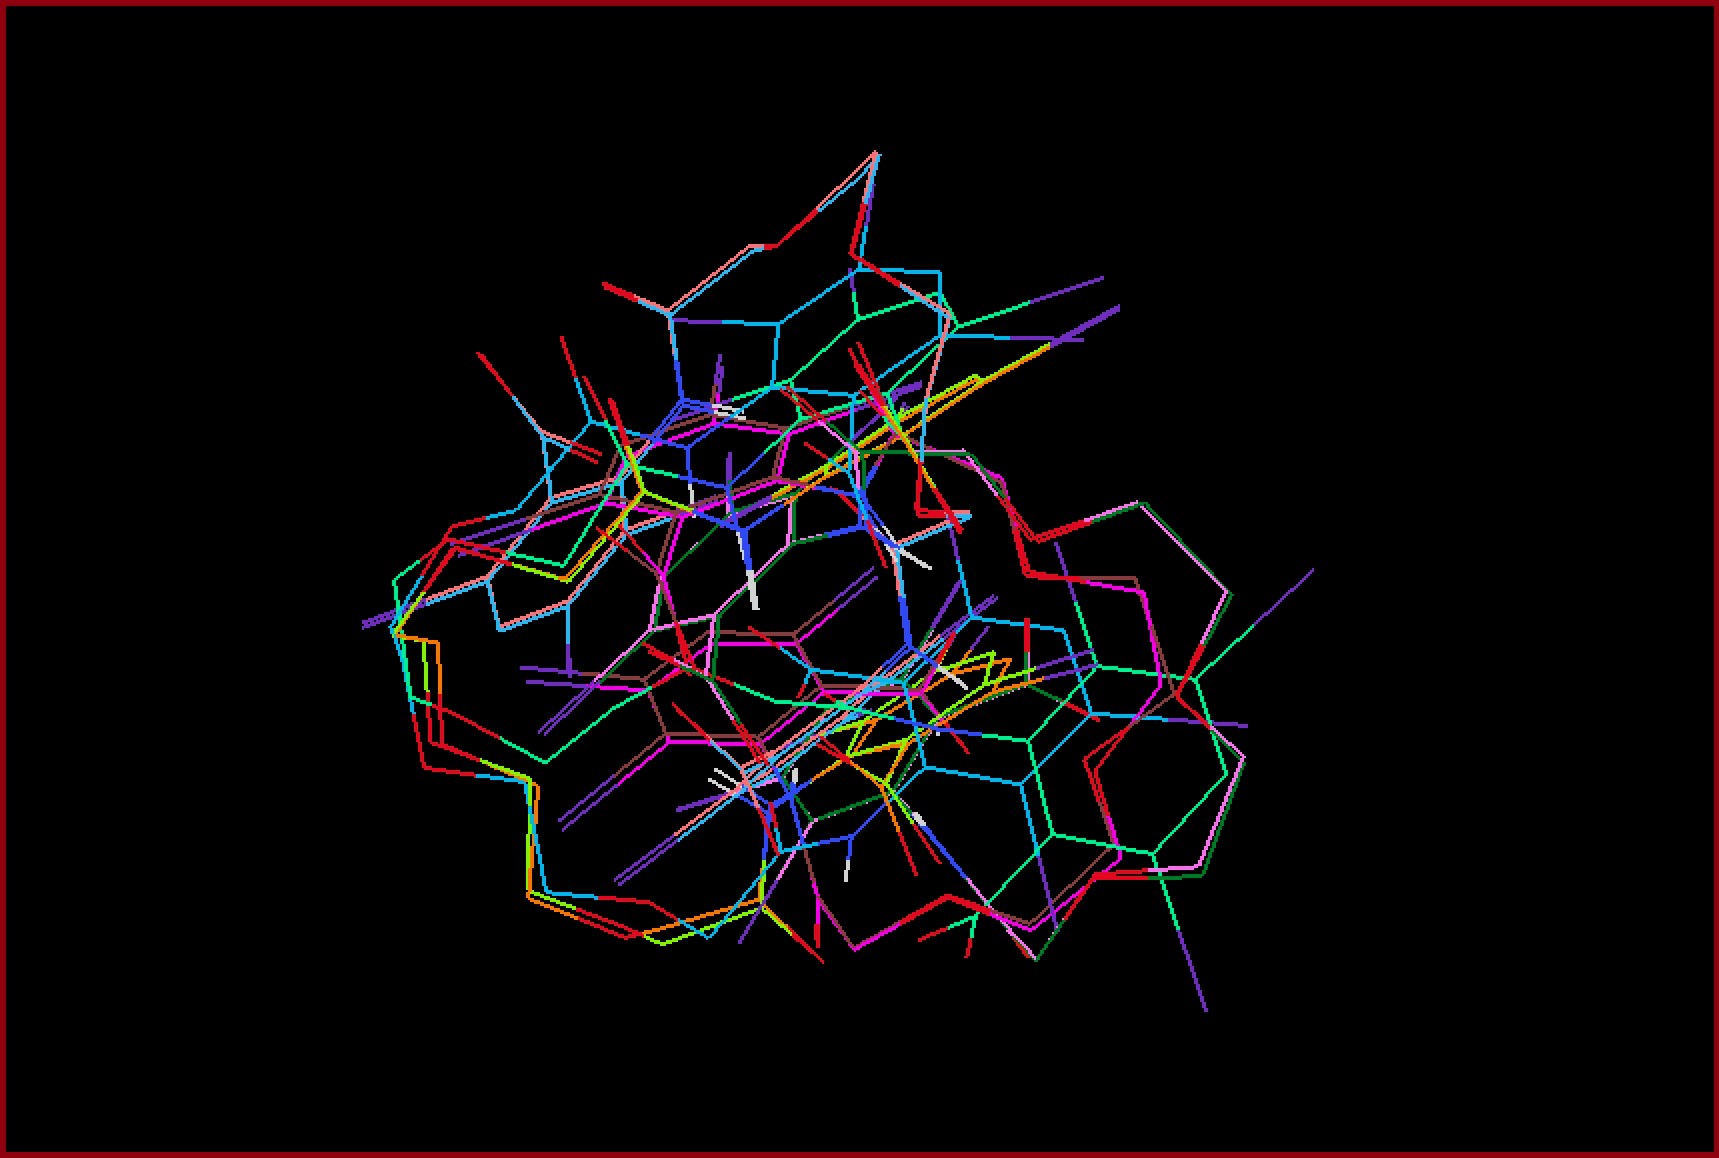
\includegraphics[width=120mm]{lig}
     \caption{Molecular model of meglumine iotroxate, designated as a World Health Organization essential medicine, visualized using AutoDockingTools \cite{autodock}.}
     \label{fig:lig}
   \end{figure} 
  
  The SMILES representation of a ligand uses symbols to describe which atoms are in the molecule, whether or not they are aromatic, which bonds are shared between them, and what charges they have as well as identifying structures such as chains, branches, and rings \cite{smiles}. In my fingerprinting algorithm I reverse the symbols in the SMILES representation to generate a table cataloging the number of atoms of each type, the number of bonds of each type, the rings, etc. After generating this SMILES fingerprinting function, I ran this function on each of the ligands in the S-protein dataset and in the S-protein:ACE2 interface dataset and replaced the SMILES representation in each dataframe with columns for each value in the fingerprint table. I then created input and output sets for both the S-protein and S-protein:ACE2 interface by isolating only the fingerprint columns as inputs and only the Vina scores column as outputs. For the input and output sets, I divided them randomly so that 75\% when into a training set and 25\% into a testing set, the same ratio used by Batra et al. \cite{batra}
  
   \begin{figure}
     \centering
     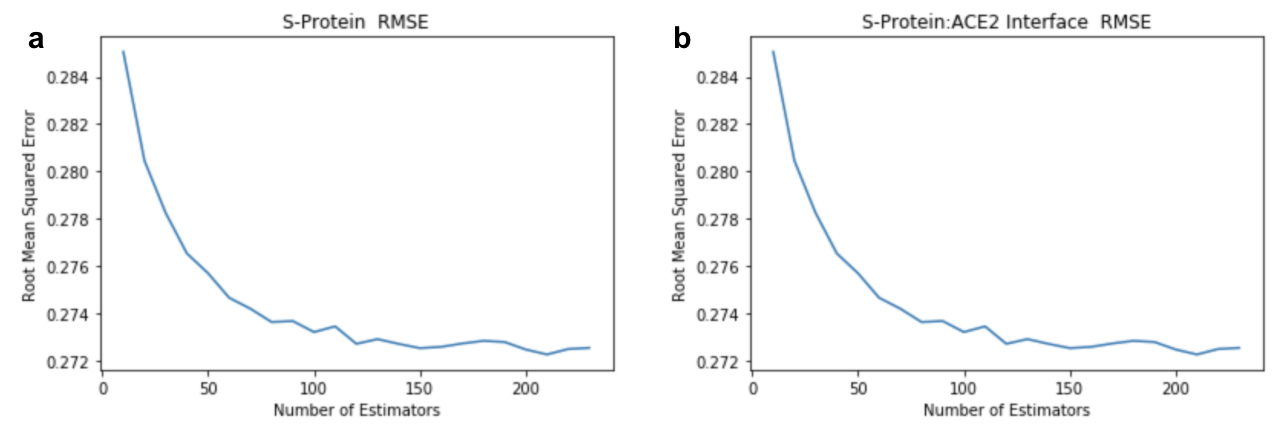
\includegraphics[width=120mm]{rferror}
     \caption{Root mean squared error associated with each number of estimators for a) the S-protein RF model and b) the S-protein:ACE2 interface RF model.}
     \label{fig:rferror}
   \end{figure} 
  
  I began by generating my own RF models to compare with Batra's model. This model, like with Batra's, uses scikit learn to build a ``forest", or an ensemble of decision trees merged together, to get more accurate and stable prediction than any single decision tree \cite{scikit}. This ensemble method is usually fast and accurate, making it one of the most popular choices for ML regression models. To tune my RF, I varied the number of estimators, or number of trees, in each model and visualized the root mean squared error for each number of estimators, given in Figure \ref{fig:rferror}. From these visualizations I determined that I could minimize the error with the fewest estimators if I set both models to have approximately 120 estimators.
  
  After generating my RF models, then used scikit learn's gradient boosting model with the same training and testing sets as the RF model \cite{scikit}. Like RF, GB is an ensemble model which combines a set of weak learners. By combining these, this GB model increases its accuracy and stability \cite{gbmodel}. To tune my GB model I used scikit learn's GridSearchCV method to scan through the learning rate, the maximum depth of a tree, the number of features to consider while searching for a best split, the minimum number of samples required in a node to be considered for splitting, and the number of estimators to find the optimal parameters for each model. After tuning these hyper parameters, I visualized the dependence of the S-protein and the S-protein:ACE2 interface on each individual variable in the fingerprint table, as shown in Figure \ref{fig:vardep}. 
  
   \begin{figure}
     \centering
     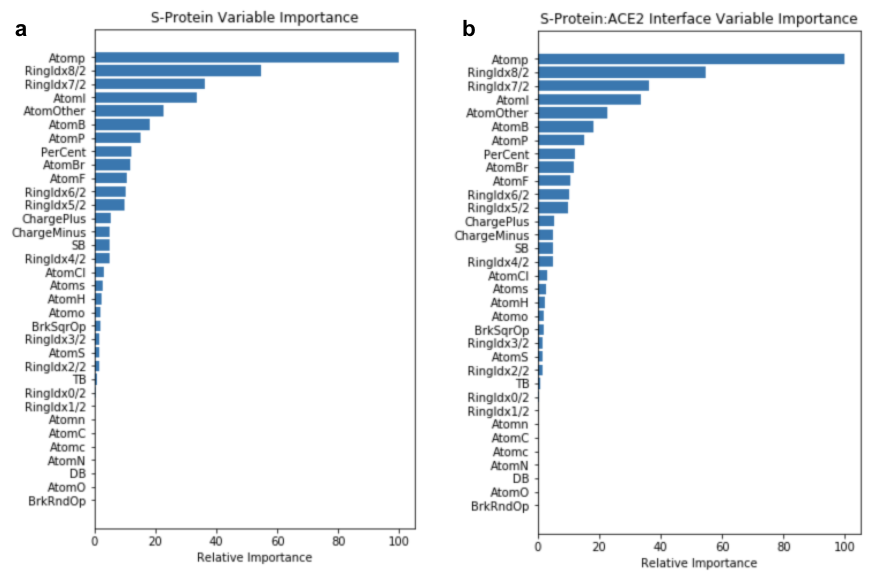
\includegraphics[width=130mm]{vardep}
     \caption{Plot of the relative feature importance of each ligand's chemical and geometric variables for a) the S-protein model and b) the S-protein:ACE2 interface model.}
     \label{fig:vardep}
   \end{figure} 
  
  After the GB models, I used scikit learn's support vector regression and kernel ridge regression models \cite{scikit}. SVR differs from other regression methods in that it uses the Support Vector Machine algorithm to try to fit the best fit line with a set epislon-error threshold \cite{svrmodel}. I tuned the two free variables for SVR, the regularization parameter C and the kernel coefficient gamma, using GridSearchCV. The KRR model shares the same form as the SVR model, but unlike SVR it sues ridge loss rather than epsilon-insensitive loss \cite{krrmodel}. I again used GridSearchCV to tune the free parameters, one variable for reducing the variance of the estimates called alpha and another kernel coefficient called gamma.
  
  The final model I created was one which stacks the output of the RF, GB, and SVR models \cite{scikit}. While this model greatly increases runtime, it inherits the strengths of each individual estimator and, as a result, can have better performance than any single model as a result. Therefore, if the results of the stacking algorithm is significantly better than any of the individual models, the increased accuracy may outweigh the increased runtime when predicting the Vina scores of a larger database of ligands. 
    
  \section{Results}
  \subsection{Verifying the Efficiency of the RF Models}
  The goal for developing these models was to verify that the RF models gave the most accurate predictions in the least amount of time. If this is the case, then Batra's virtual screening method would need no further changes. While my models differ sightly from Batra's, as I did not have access to the hyperparameters or fingerprinting algorithms used in his research, the development of my own models should provide a baseline to determine whether or not his assumption that an RF model would perform best is sound. 
  
  Figure \ref{fig:rf} presents the performance results of the S-protein and S-protein:ACE2 interface RF models on the Smith dataset. Both models have relatively good performance on the test set with a MSE of 0.07 kcal/mol for the S-protein model and a MSE of 0.56 kcal/mol for the S-protein:ACE2 interface.
    
   \begin{figure}
     \centering
     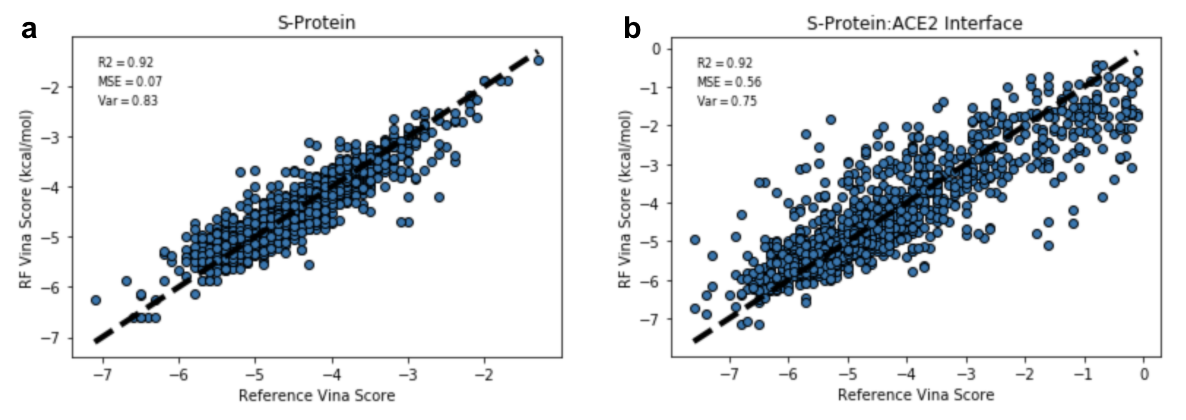
\includegraphics[width=160mm]{rf}
     \caption{Parity plot of the a) S-protein and b) S-Protein:ACE2 interface RF models for the test set, both demonstrating good prediction accuracy.}
     \label{fig:rf}
   \end{figure} 
  
  Comparing the performance of this RF model to the model used by Batra, we see that this RF model performs approximately the same, if not marginally better, than the model used in his work which had a MSE of 0.08 kcal/mol for the S-protein and 0.71 kcal/mol for the S-protein:ACE2 interface, as shown in Figure \ref{fig:batraRF}.
  
   \begin{figure}
     \centering
     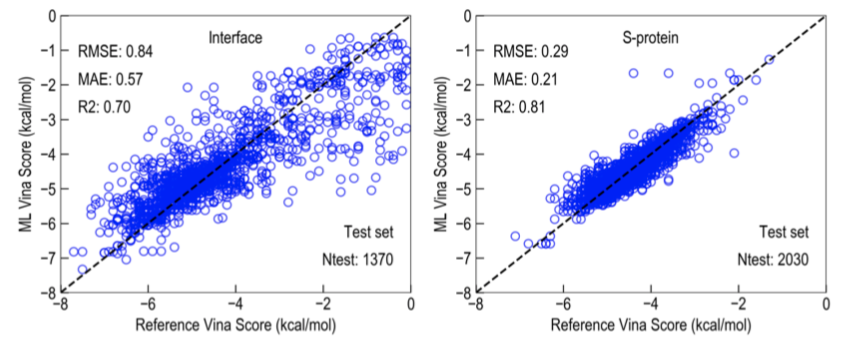
\includegraphics[width=160mm]{batraRF}
     \caption{Parity plot used in the analysis performed by Batra et al. for the S-protein and S-Protein:ACE2 interface RF models on the test set, both demonstrating good prediction accuracy, if not marginally worse than my model for the S-protein:ACE2 interface \cite{smith}.}
     \label{fig:batraRF}
   \end{figure} 
   
   The performance of the GB model for the S-protein and the S-protein:ACE2 interface on the Smith dataset is given in Figure \ref{fig:gb}. We see that the results of these models are virtually identical to those of my RF models, with a MSE of 0.07 kcal/mol for the S-protein model and a MSE of 0.57 kcal/mol for the S-protein:ACE2 interface model. While this model performed identically to the RF model, it took significantly longer to tune the GB model compared to the RF model.
   
   \begin{figure}
     \centering
     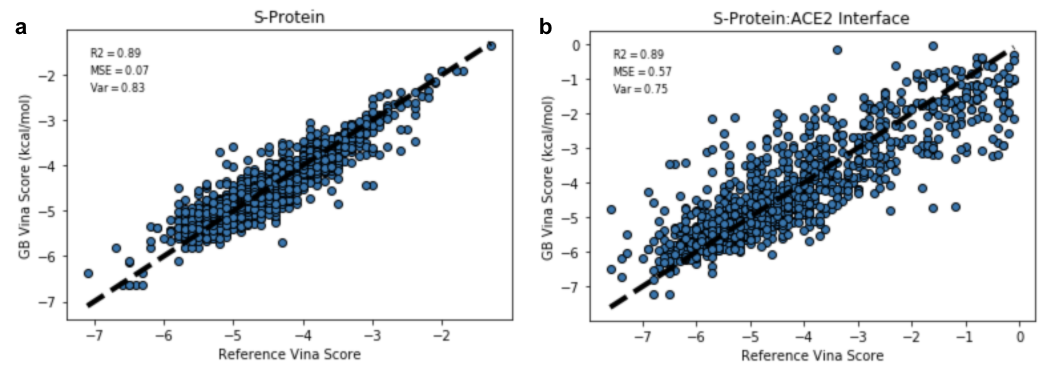
\includegraphics[width=160mm]{gb}
     \caption{Parity plot of the a) S-protein and b) S-Protein:ACE2 interface GB models for the test set, both demonstrating similar accuracy levels to the RF model.}
     \label{fig:gb}
   \end{figure} 
      
   Figure \ref{fig:svr} displays the performance of the SVR model for the S-protein and interface. For the S-protein the SVR model performance is nearly identical to that of the above models, with a MSE of 0.08 kcal/mol, but for the S-protein:ACE2 interface the SVR model performed marginally worse, with a MSE of 0.64 kcal/mol. 
   
   \begin{figure}
     \centering
     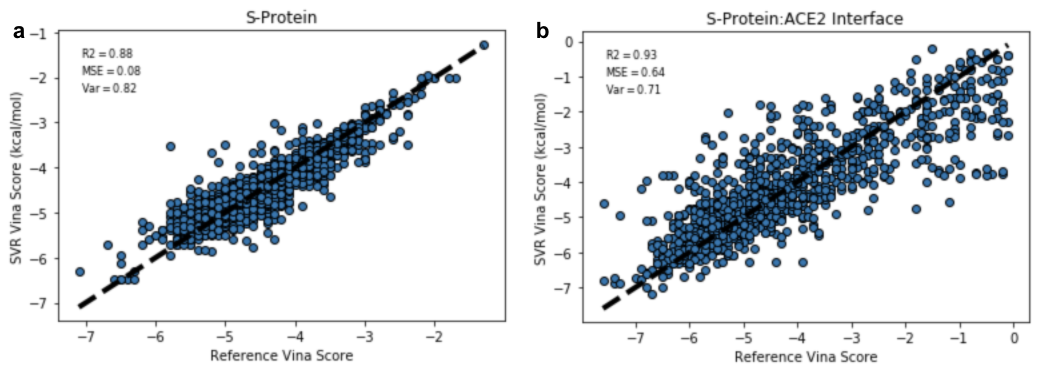
\includegraphics[width=160mm]{svr}
     \caption{Parity plot of the a) S-protein and b) S-Protein:ACE2 interface SVR models for the test set, demonstrating an accuracy that is on par with RF for the S-protein and marginally worse for the interface.}
     \label{fig:svr}
   \end{figure} 
   
   Figure \ref{fig:krr} displays the performance of the KRR model for the S-protein and interface. This model is marginally worse than the RF for both, with a MSE of 0.10 kcal/mol for the S-protein model and a MSE of 0.65 kcal/mol for the S-protein:ACE2 interface model. 
   
   \begin{figure}
     \centering
     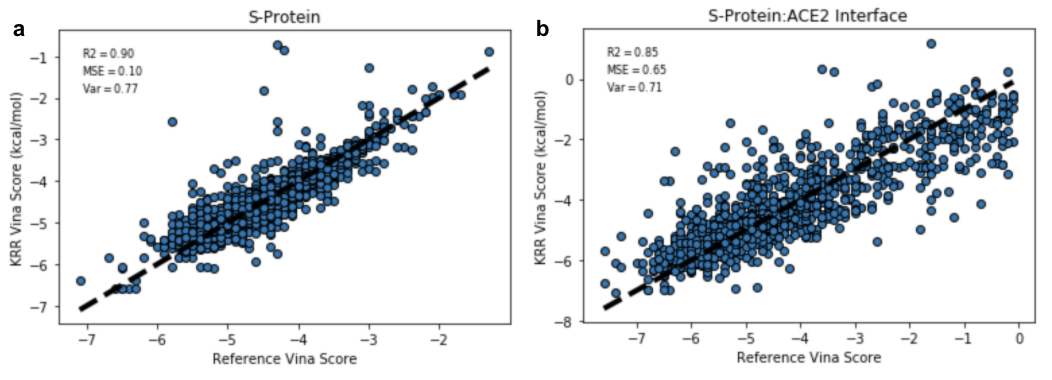
\includegraphics[width=160mm]{krr}
     \caption{Parity plot of the a) S-protein and b) S-Protein:ACE2 interface KRR models for the test set, both with an accuracy that is slightly worse than the RF model.}
     \label{fig:krr}
   \end{figure} 
   
   The performance of the final model, which stacks the RF, GB, and SVR models, is displayed in Figures \ref{fig:iso} and \ref{fig:int}. Noice that there are some differences between the RF, GB, and SVR models used in the stacking which are due to differences between my custom hyperparameter tuning and the tuning performed by the stacking algorithm. While the stacked model performs just as well as the other models for the S-protein:ACE2 interface and marginally worse for the S-protein, with a MSE of 0.21 kcal/mol for the S-protein model and a MSE of 0.56 kcal/mol for the S-protein:ACE2 interface model, there is no jump in improvement to justify the increase in runtime.
  
   \begin{figure}
     \centering
     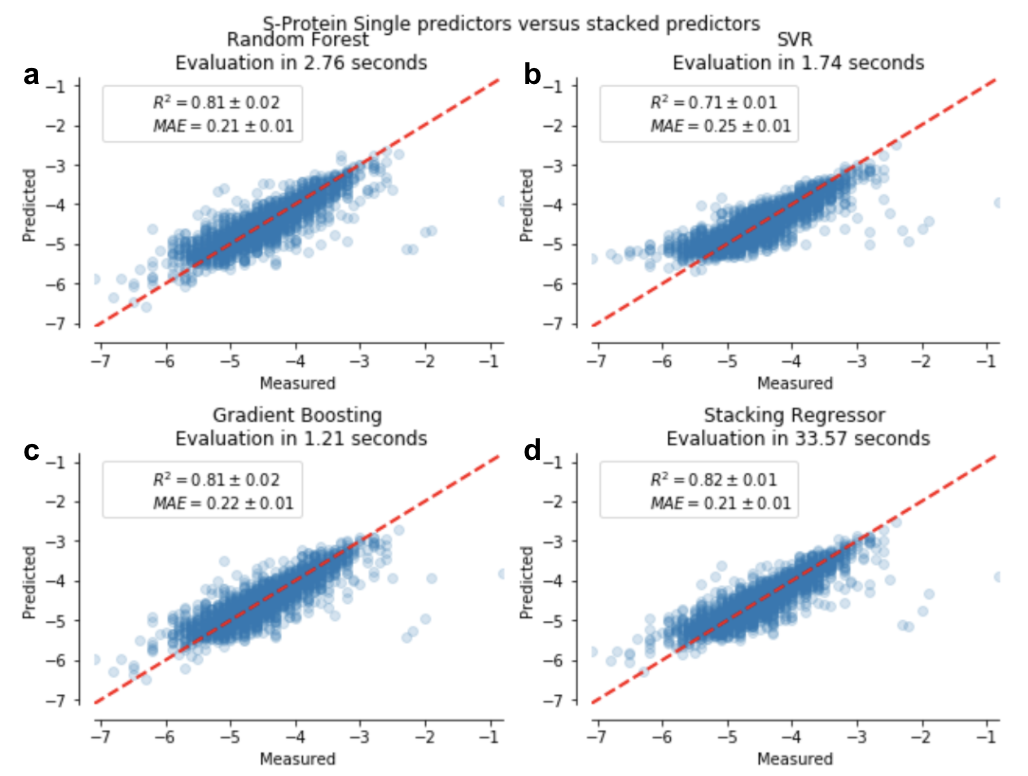
\includegraphics[width=120mm]{isoStacked}
     \caption{Parity plots generated by the scikit learn stacking algorithm for the S-protein a) RF, b) GB, c) SVR, and d) stacked models for the test set, demonstrating marginally worse prediction accuracy than the RF model and with a significantly longer runtime \cite{scikit}.}
     \label{fig:iso}
   \end{figure} 
   
   \begin{figure}
     \centering
     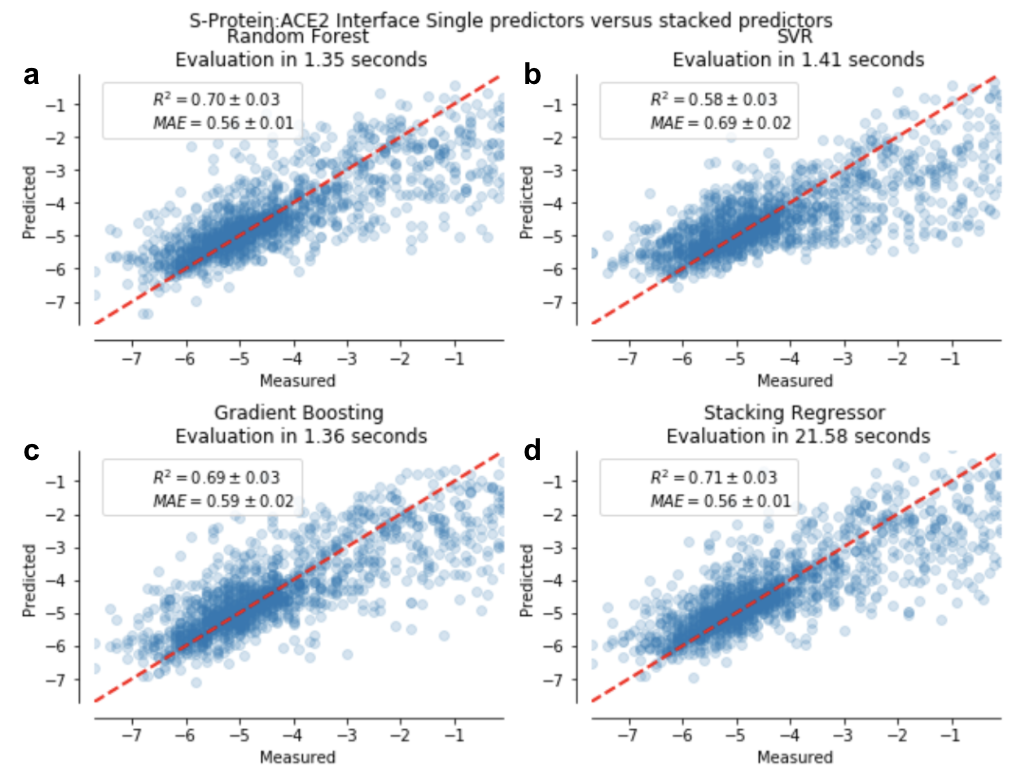
\includegraphics[width=120mm]{intStacked}
     \caption{Parity plots generated by the scikit learn stacking algorithm for the S-protein:ACE2 interface a) RF, b) GB, c) SVR, and d) stacked models for the test set, demonstrating good prediction accuracy as compared to the RF model but with a significantly longer runtime \cite{scikit}.}
     \label{fig:int}
   \end{figure} 
   
   We see from these results that the RF model does minimize the error for the both the S-protein and the S-protein:ACE2 interface, with a mean squared error of 0.07 kcal/mol for the S-protein and with a mean squared error of 0.56 kcal/mol for the S-protein:ACE2 interface. The only other models which match these errors, gradient boosting for the S-protein and stacking for the S-protein:ACE2 interface, take significantly longer to run, making the RF model the optimal choice here. 
   
   \subsection{RF-based Screening of Ligands}
   The results of these tests indicate that for further screening the best choice of ML model is the RF regressor, which was optimized in the section above. Because this model was both the fastest and most efficient, it allowed us to quickly screen through new ligand candidates as quickly and accurately as possible. My model varies from the models used by Smith and Batra, so using the RF models I developed should help to identify additional strongly binding ligands for the S:protein or S:protein:ACE2 interface. To find these  ligands, I used the RF model to make predictions about the Vina scores of the FDA approved active ingredients in the CureFFI dataset and other ligands in the DrugCentral dataset, which do not have known Vina scores. Predicting the Vina scores on the same dataset as Batra with the same screening criteria (given by the equation $y$=$-\frac{x}{2} - 7.5$ where $x$ represents the S-protein:ACE2 interface Vina scores and $y$ represents the S-protein Vina scores) we can see visually that significantly fewer ligands passed the screening criteria for both the FDA approved ligands and the other ligands using my model as compared with the model developed by Batra et al, demonstrated in Figures \ref{fig:myScreen} and \ref{fig:batraScreen}.
   
   \begin{figure}
     \centering
     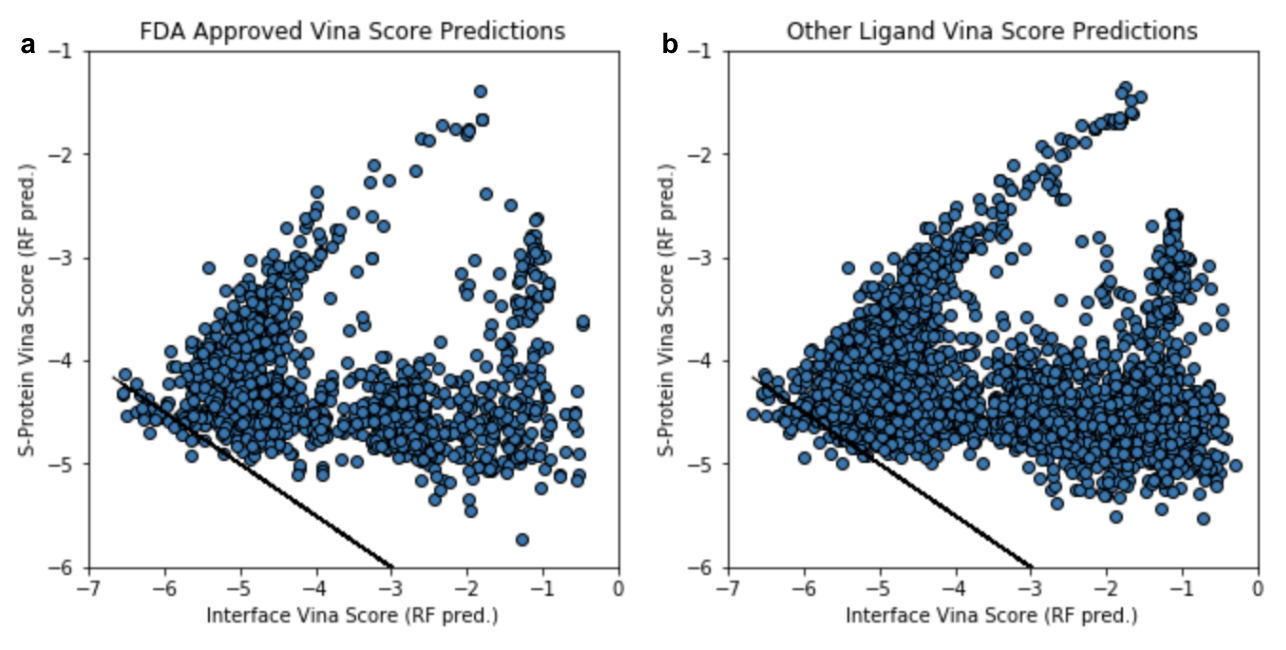
\includegraphics[width=120mm]{myscreening}
     \caption{RF predictions of the Vina scores for the S-protein against the RF predictions of the Vina scores for the S-protein:ACE2 interface for a) FDA approved ligands, and b) other ligands as generated by my RF model.}
     \label{fig:myScreen}
   \end{figure} 

   \begin{figure}
     \centering
     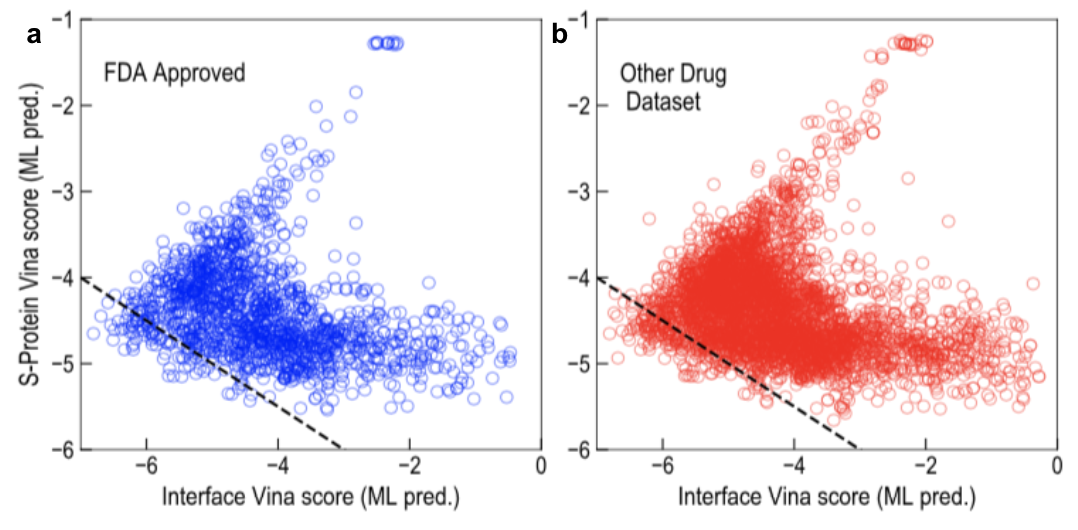
\includegraphics[width=120mm]{batrascreening}
     \caption{RF predictions of the Vina scores for the S-protein against the RF predictions of the Vina scores for the S-protein:ACE2 interface for a) FDA approved ligands, and b) other ligands as generated by the RF model presented in Batra et al.}
     \label{fig:batraScreen}
   \end{figure} 
   
  Numerically, we see that only 64 ligands passed Batra's screening test with 21 FDA approved ligands passing the screening and 43 others. This is slightly more than $\frac{1}{3}$ the total number of ligands passing the test using the model generated by Batra et al. Among these 64 ligands, only two of the FDA approved ligands and only one of the other ligands were common to Batra's top candidates, and only the non-FDA approved ligand perflubron was common with Smith's top candidates. In order to increase the number of drugs passing the screening, I eased the screening cut to $y$=$-\frac{x}{2} - 7.3$. This resulted in the top candidates listed in Figure \ref{fig:topcandidates}.
  
  \begin{figure}
     \centering
     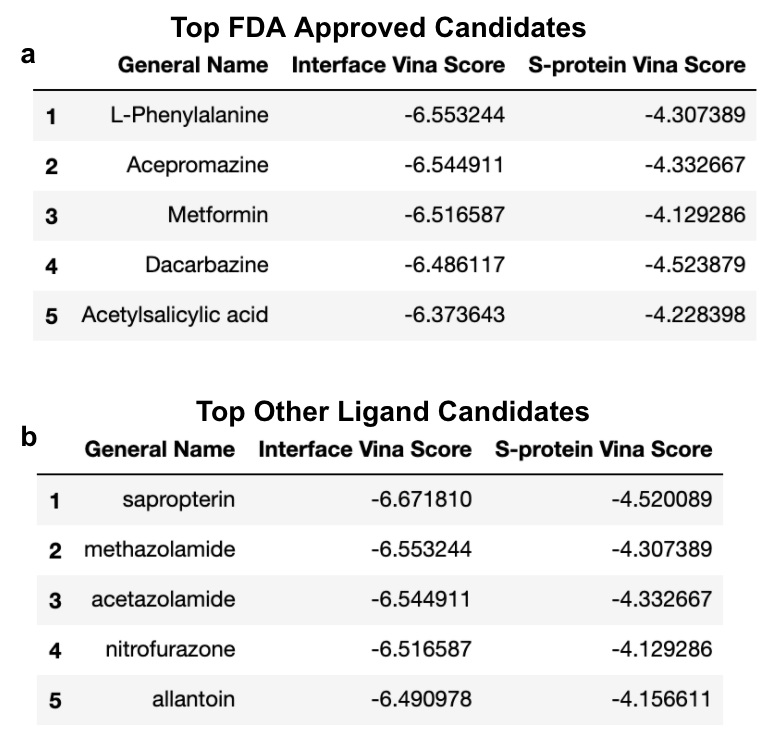
\includegraphics[width=80mm]{topcandidates}
     \caption{Top ligand candidates passing my therapeutic ligand screening cuts organized as a) FDA approved ligands from the CureFFI dataset and b) other ligands from the DrugCentral dataset \cite{cureffi,drugcentral}}
     \label{fig:topcandidates}
   \end{figure}
   
      Among the FDA approved ligands the top candidate is the essential amino acid L-Phenylalanine, found in dietary sources like meat, fish, eggs, cheese, and milk. Its 3D molecular structure is given in Figure \ref{fig:phen}. Its role in the human body is not fully understood, but it plays a key role in the biosynthesis of other amino acids and in the function of many proteins and enzymes \cite{pubChemLPhen}. Among the non-FDA approved ligands the top candidate is sapropterin, a cofactor in the synthesis of nitric oxide. It is essential for the conversion of phenylalanine to tyrosine, and its 3D molecular structure is given in Figure \ref{fig:sapro} \cite{drugbank}.
  
   \begin{figure}
     \centering
     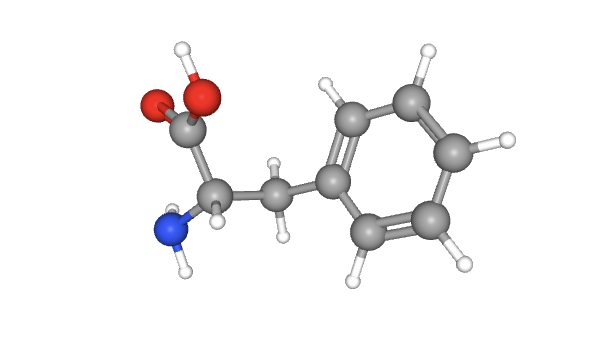
\includegraphics[width=100mm]{phen}
     \caption{3D structure of L-phenylalanine, the top candidate of the FDA approved ligands \cite{pubChemLPhen}.}
     \label{fig:phen}
   \end{figure}
   
   \begin{figure}
     \centering
     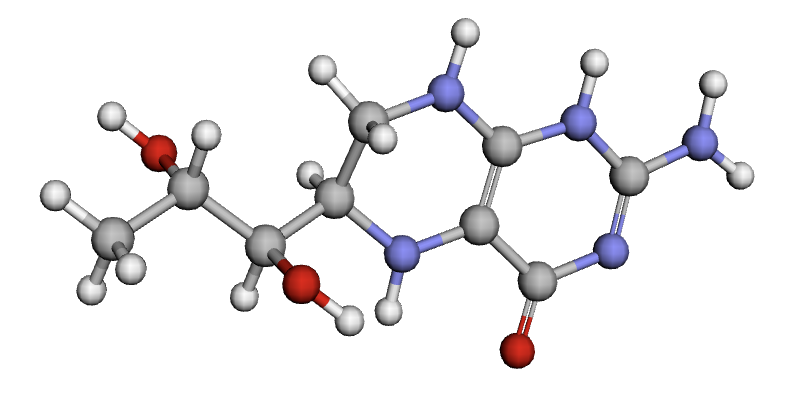
\includegraphics[width=100mm]{sapro}
     \caption{3D structure of sapropterin, the top candidate of the non-FDA approved ligands \cite{drugbank}.}
     \label{fig:sapro}
   \end{figure}

  
  \section{Conclusion}
  To help recover from the COVID-19 pandemic, both in terms of health and economics, it is crucial that a treatment be discovered and approved in a timely manner. This can only happen with more sophisticated treatment discovery methods than trial and error, and scientists have turned to virtual screening to help narrow their search for suitable therapeutic treatments. In this paper, I verified the assumption presented by Batra et al. that the random forest model is the most effective machine learning (ML) model for the virtual screening of ligands with the potential to limit or disrupt the host-virus interactions for COVID-19 \cite{batra}. Under the assumption that ligands which bind most strongly to the spike proteins (S-proteins) on the viral cells or to the S-protein and human Angiotensin-converting enzyme 2 (ACE2) receptor complex are likely to be the most effective treatments, I developed five ML models - random forest (RF), gradient boosting (GB), support vector regressor (SVR), kernel ridge regressor (KRR), and RF, GB, and SVR stacked regressor - to predict Vina scores based on  geometric and chemical information characterizing the ligand. To train the ML models, used the dataset generated by autodocking simulations  performed by Smith et al. and used a chemical fingerprinting algorithm to convert the SMILES representation of each ligand into a table of geometric and chemical features of the molecule \cite{schwartz,smith}. I found that my RF model performed equally as well if not better at minimizing error than all other regression models, with a mean squared error of 0.07 kcal/mol for the S-protein model and 0.56 kcal/mol for the S-protein:ACE2 interface model, and had a significantly faster runtime. Using this RF model, I predicted the Vina scores for the ligands in the CureFFI and DrugCentral datasets and used a simple screening function to identify those with the lowest Vina scores. Among those which passed the screening, I was able to identify the top five treatment candidates for both the datasets. While I could not verify the rank-ordering of of the BindingDB dataset generated in Batra et al. due to computational constraints, the similarity in the errors between my RF models and Batra's suggests that there would not be much change in the overall ranking \cite{batra,cureffi,bindingdb,drugcentral}.
  
   \newpage
    
    \begin{thebibliography}{9}
    
\bibitem{smiles} 
Anderson, E., G.D. Veith, and D. Weininger.
\textit{SMILES: A line notation and computerized interpreter for chemical structures}.
Report No. EPA/600/M-87/021. U.S. Environmental Protection Agency, Environmental Research Laboratory-Duluth, Duluth, MN 55804, 1987.

\bibitem{batra} 
Rohit Batra, Henry Chan, Ganesh Kamath, Rampi Ramprasad, Mathew J. Cherukara, and Subramanian Sankaranarayanan.
\textit{Screening of Therapeutic Agents for COVID-19 using Machine Learning and Ensemble Docking Simulations}.
April 2020.

\bibitem{cureffi} 
CureFFI.
\url{https://www.cureffi.org/2013/10/04/list-of-fda-approved-drugs-and-cns-drugs-with-smiles/}

\bibitem{drugbank}
Drugbank.
\textit{Sapropterin}.
\url{https://www.drugbank.ca/drugs/DB00360}


\bibitem{bindingdb} 
Michael K Gilson, Tiqing Liu, Michael Baitaluk, George Nicola, Linda Hwang, and Jenny Chong.
\textit{BindingDB in 2015: a public database for medicinal chemistry, computational chemistry and systems pharmacology}.
Nucleic acids research, 44(D1):D1045–D1053, 2016.
\url{https://www.bindingdb.org/bind/index.jsp}

\bibitem{autodock} 
Morris, G. M., Huey, R., Lindstrom, W., Sanner, M. F., Belew, R. K., Goodsell, D. S. and Olson, A. J.R.
\textit{Autodock4 and AutoDockTools4: automated docking with selective receptor flexiblity}.
J. Computational Chemistry 2009, 16: 2785-91.

\bibitem{pubChemLPhen}
National Center for Biotechnology Information.
PubChem Database. Phenylalanine, CID=6140.
\url{https://pubchem.ncbi.nlm.nih.gov/compound/Phenylalanine}

\bibitem{scikit} 
Pedregosa et al.
\textit{Scikit-learn: Machine Learning in Python}.
JMLR 12, pp. 2825-2830, 2011.

\bibitem{krrmodel} 
Niranjan Pramanik.
\textit{Kernel Regression — with example and code}.
Towards Data Science, Sep. 2019.

\bibitem{mlmodels}
Matthew C. Robinson, Robert C. Glen, and Alpha A. Lee.
\textit{Validating the Validation: Reanalyzing a large-scale comparison of Deep Learning and Machine Learning models for bioactivity prediction}.
9 June, 2019.

\bibitem{schwartz}
Julian Schwartz, Mahendra Awale and Jean-Louis Reymond.
\textit{The SMIfp (SMILES fingerprint) Chemical Space for Virtual Screening and Visualization of Large Databases of Organic Molecules}.
J. Chem. Inf. Model. July 2013, 53, 8, 1979-1989.

\bibitem{virtualscreening}
Kanishka S Senathilake, Sameera R Samarakoon, Kamani H Tennekoon.
\textit{Virtual screening of inhibitors against spike glycoprotein of 2019 novel corona virus: a drug repurposing approach}.
Preprints 2020, 2020030042.

\bibitem{svrmodel}
Tom Sharp.
\textit{An Introduction to Support Vector Regression (SVR)}.
Towards Data Science, Mar. 2020.

\bibitem{gbmodel}
Harshdeep Singh.
\textit{Understanding Gradient Boosting Machines}.
Towards Data Science, Nov. 2018.

\bibitem{smith} 
Micholas Smith and Jeremy C. Smith.
\textit{Repurposing therapeutics for covid-19: Supercomputer-based docking to the sars-cov-2 viral spike protein and viral spike protein-human ace2 interface}.
Feb 2020.

\bibitem{drugcentral} 
Oleg Ursu, Jayme Holmes, Jeffrey Knockel, Cristian G Bologa, Jeremy J Yang, Stephen L Mathias, Stuart J Nelson, and Tudor I Oprea.
\textit{DrugCentral: online drug compendium}.
Nucleic acids research, page gkw993, 2016.
\url{http://drugcentral.org/}

\end{thebibliography}  
 
  
%%%%%%%%%%%%%%%%%%%%%%%%%%%%%%%%%%%%%%%%%%%%%%%%%%%%%%%%%%%%%%%%%  
\end{document}